%
% Capítulo 1
%
\chapter{Introdução} \label{cap:intro}

A maioria dos domicílios, lojas e escritórios recorrem a serviços de abastecimento de água. O custo deste serviço é usualmente calculado através da estimativa da quantidade de água gasta (por norma mensalmente) e, periodicamente, um funcionário da empresa prestadora do serviço tem de se deslocar à localização do contador para que seja verificado o consumo real de água para o acerto do pagamento.\par
A evolução tecnológica dos últimos anos tem facilitado e incentivado o acesso de grande parte das pessoas aos vários equipamentos e plataformas tecnológicas que nos permitem efetuar diversas tarefas que outrora necessitariam de outra burocracia ou até serviço presencial. A entrega da leitura da contagem da água é algo que pode ser modernizado e automatizado. Porém reconhecemos que soluções que envolvam, por exemplo, a substituição dos equipamentos contadores, possam acarretar um custo logístico e financeiro não justificável para o fornecedor do serviço. \par
Neste projeto, foi desenvolvido um sistema informático que pretende solucionar os problemas apresentados, modernizando o processo de entrega de leituras de água. \par
A figura \ref{fig:interacoes}  representa as interações do sistema Water Watcher, bem como os elementos com os quais o sistema interage.

\begin{figure}[h!]
\begin{center}
\resizebox{80mm}{!}{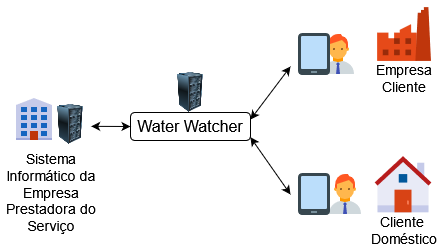
\includegraphics{diagramas/wws.png}}
\caption{Interações do sistema.}
\label{fig:interacoes}
\end{center}
\end{figure}

\vspace{1cm}

Como podemos observar na figura, o sistema Water Watcher é um sistema complementar ao sistema que a empresa prestadora do serviço de fornecimento de água já utiliza para gerir os clientes e as suas contagens, pelo que, caso implementado, seria gerido por esta empresa.\par
Este sistema comunica com os utilizadores através de uma interface, à qual podem aceder através de um dispositivo com acesso a um \textit{web browser} e comunica também com o sistema do prestador de serviços para obter e fornecer informações sobre os utilizadores.

%
% Secção 1.1
%
\section{Objetivo do Projeto} \label{sec11}

De forma a não ser necessário proceder a acertos de pagamentos e permitir que o cliente pague realmente o valor que consumiu, ao invés do consumo estimado, este projeto teve como propósito o desenvolvimento de um sistema informático composto por, de entre outros elementos, um elemento que o cliente utiliza para comunicar ao fornecedor o seu consumo de água. Este sistema interagirá com o sistema informático já utilizado pela empresa prestadora do serviço para a gestão das contagens de água dos clientes, pelo que será mantido também por esta entidade. Este poderá também ser utilizado para apresentar estatísticas de consumo e notificar o cliente sobre informações pertinentes relativas a este serviço. Para além deste elemento, também vai ser realizado um servidor cuja função principal é comunicar com o elemento dos utilizadores e interagir com o local onde estão guardadas as informações dos clientes.

\section{Organização do Documento} \label{sec12}

O restante relatório encontra-se organizado em quatro capítulos. No capítulo \ref{cap:trabrelacionado} vamos avaliar e debater soluções já existentes no mercado cuja função se aproxima da do sistema desenvolvido neste projeto, bem como os vários equipamentos e conceitos utilizados na área cujo projeto se insere. No capítulo \ref{cap:analise} são analisados os vários problemas do projeto, detalhando os vários requisitos que o sistema terá de cumprir para satisfazer o seu propósito. No capítulo \ref{cap:abordagem} são estudadas as várias abordagens aos problemas do projeto. No capítulo \ref{cap:implementacao} são analisadas as várias escolhas e decisões que foram efetuadas no desenvolvimento deste projeto.\par
No repositório Github \texttt{https://github.com/AteBreves/PS} estão todos os recursos desenvolvidos neste projeto, como os ficheiros de texto e imagens que compõem este relatório e todo o código do sistema Water Watcher.

%O capítulo \ref{cap:trabrelacionado} será onde vamos comparar e explicar as várias estratégias de abordagem às soluções apresentadas.
% Por fim, o capítulo 5 (Aspetos de Implementação) será onde vamos analisar diretamente o código fonte da solução e explicar os diversos detalhes e escolhas efetuadas durante a escrita do código.